\section{Additional boards analysis} % (fold)
\label{app:additional_error_plots}

\subsection{Right high density trap-distributed board}

The board used in this case is the following (figure~\ref{fig:board_right}).

\begin{figure}[H]
\centering
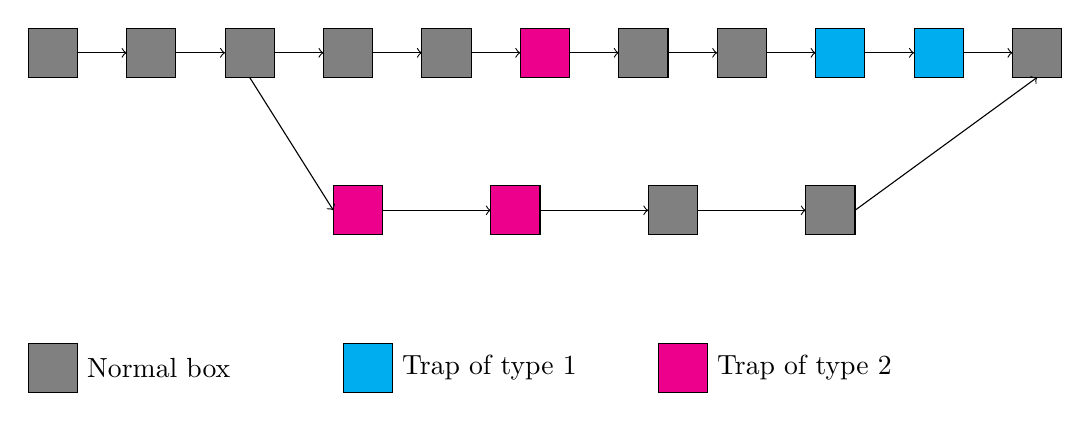
\begin{tikzpicture}[scale=10]
%board = [0,0,0,0,0,2,0,0,1,1,2,2,0,0,0]
\pgfmathsetmacro{\i}{1-1}
\pgfmathsetmacro{\c}{"gray"}
\draw [fill=\c] (2*\i*0.0625,1) rectangle (2*\i*0.0625+0.0625,1-0.0625);
\pgfmathsetmacro{\i}{2-1}
\pgfmathsetmacro{\c}{"gray"}
\draw [fill=\c] (2*\i*0.0625,1) rectangle (2*\i*0.0625+0.0625,1-0.0625);
\pgfmathsetmacro{\i}{3-1}
\pgfmathsetmacro{\c}{"gray"}
\draw [fill=\c] (2*\i*0.0625,1) rectangle (2*\i*0.0625+0.0625,1-0.0625);
\pgfmathsetmacro{\i}{4-1}
\pgfmathsetmacro{\c}{"gray"}
\draw [fill=\c] (2*\i*0.0625,1) rectangle (2*\i*0.0625+0.0625,1-0.0625);
\pgfmathsetmacro{\i}{5-1}
\pgfmathsetmacro{\c}{"gray"}
\draw [fill=\c] (2*\i*0.0625,1) rectangle (2*\i*0.0625+0.0625,1-0.0625);
\pgfmathsetmacro{\i}{6-1}
\pgfmathsetmacro{\c}{"magenta"}
\draw [fill=\c] (2*\i*0.0625,1) rectangle (2*\i*0.0625+0.0625,1-0.0625);
\pgfmathsetmacro{\i}{7-1}
\pgfmathsetmacro{\c}{"gray"}
\draw [fill=\c] (2*\i*0.0625,1) rectangle (2*\i*0.0625+0.0625,1-0.0625);
\pgfmathsetmacro{\i}{8-1}
\pgfmathsetmacro{\c}{"gray"}
\draw [fill=\c] (2*\i*0.0625,1) rectangle (2*\i*0.0625+0.0625,1-0.0625);
\pgfmathsetmacro{\i}{9-1}
\pgfmathsetmacro{\c}{"cyan"}
\draw [fill=\c] (2*\i*0.0625,1) rectangle (2*\i*0.0625+0.0625,1-0.0625);
\pgfmathsetmacro{\i}{10-1}
\pgfmathsetmacro{\c}{"cyan"}
\draw [fill=\c] (2*\i*0.0625,1) rectangle (2*\i*0.0625+0.0625,1-0.0625);
\pgfmathsetmacro{\i}{11-11}
\pgfmathsetmacro{\c}{"magenta"}
\draw [fill=\c] (0.45+\i*0.2,0.8) rectangle (0.45+\i*0.2-0.0625,0.8-0.0625);
\pgfmathsetmacro{\i}{12-11}
\pgfmathsetmacro{\c}{"magenta"}
\draw [fill=\c] (0.45+\i*0.2,0.8) rectangle (0.45+\i*0.2-0.0625,0.8-0.0625);
\pgfmathsetmacro{\i}{13-11}
\pgfmathsetmacro{\c}{"gray"}
\draw [fill=\c] (0.45+\i*0.2,0.8) rectangle (0.45+\i*0.2-0.0625,0.8-0.0625);
\pgfmathsetmacro{\i}{14-11}
\pgfmathsetmacro{\c}{"gray"}
\draw [fill=\c] (0.45+\i*0.2,0.8) rectangle (0.45+\i*0.2-0.0625,0.8-0.0625);
\pgfmathsetmacro{\i}{15-5}
\pgfmathsetmacro{\c}{"gray"}
\draw [fill=\c] (2*\i*0.0625,1) rectangle (2*\i*0.0625+0.0625,1-0.0625);

\foreach \i in {0,1,...,9}
  \draw [->] (0.0625+2*\i*0.0625,1-0.03125) -- (2*0.0625+2*\i*0.0625,1-0.03125);
\foreach \i in {0,1,2}
  \draw [->] (0.45+\i*0.2,0.8-0.03125) -- (0.45+0.1375+\i*0.2,0.8-0.03125);
\draw [->] (5*0.0625-0.03125,1-0.0625) -- (0.45-0.0625, 0.8-0.03125);
\draw [->] (0.45+0.1375+2*0.2+0.0625,0.8-0.03125) -- (2*10*0.0625+0.0625/2,1-0.0625);

\draw [fill=gray] (0,0.6) rectangle (0.0625, 0.6-0.0625);
\node [right] at (0.0625, 0.6-0.03125) {Normal box};
\draw [fill=cyan] (0.4,0.6) rectangle (0.4 + 0.0625, 0.6-0.0625);
\node [right] at (0.4 + 0.0625, 0.6-0.03125) {Trap of type 1};
\draw [fill=magenta] (0.8,0.6) rectangle (0.8 + 0.0625, 0.6-0.0625);
\node [right] at (0.8 + 0.0625, 0.6-0.03125) {Trap of type 2};
\end{tikzpicture}
\caption{Representation of our high right density trap-distributed board.}
\label{fig:board_right}
\end{figure}

The results graphs are as follows 
(figures~\ref{fig:cost_iterations_log_right}, \ref{fig:cost_per_square_100_iter_right}
and~\ref{fig:cost_subopt_log_right}).

\begin{figure}[H]
\centering
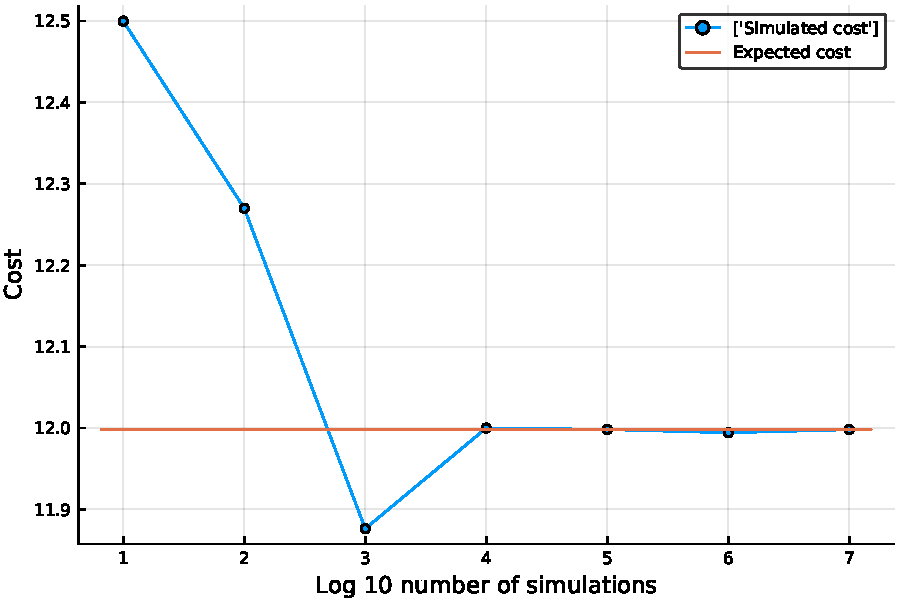
\includegraphics[scale=0.53]{../img/board_right_high/cost_iterations_log_noncirc.pdf}
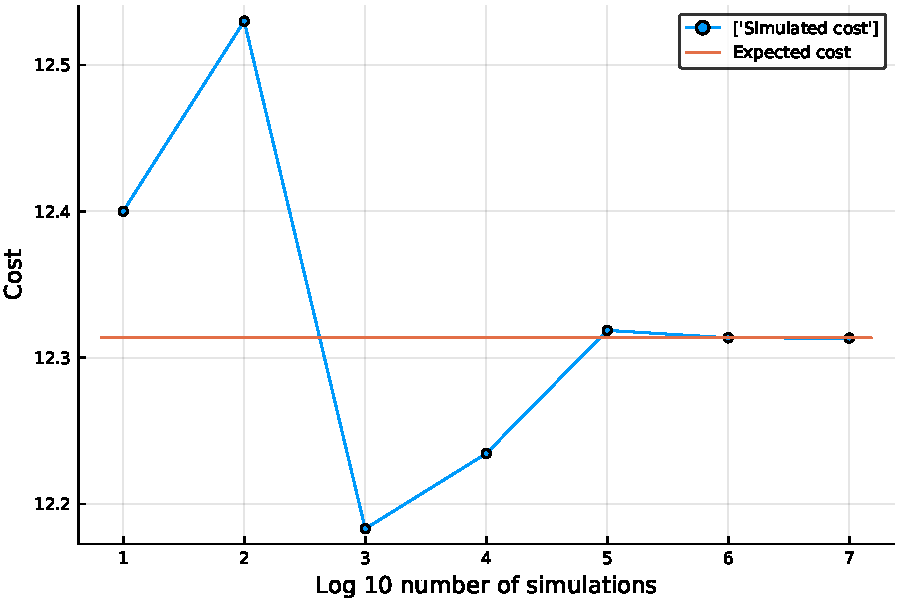
\includegraphics[scale=0.53]{../img/board_right_high/cost_iterations_log_circ.pdf}
\caption{Evolution of the simulated cost with the number of simulations. The horizontal line represent the expected cost computed with the value-iteration algorithm. On the left, results for the non-circular configuration. On the right, the circular one.}
\label{fig:cost_iterations_log_right}
\end{figure}

\begin{figure}[H]
\centering
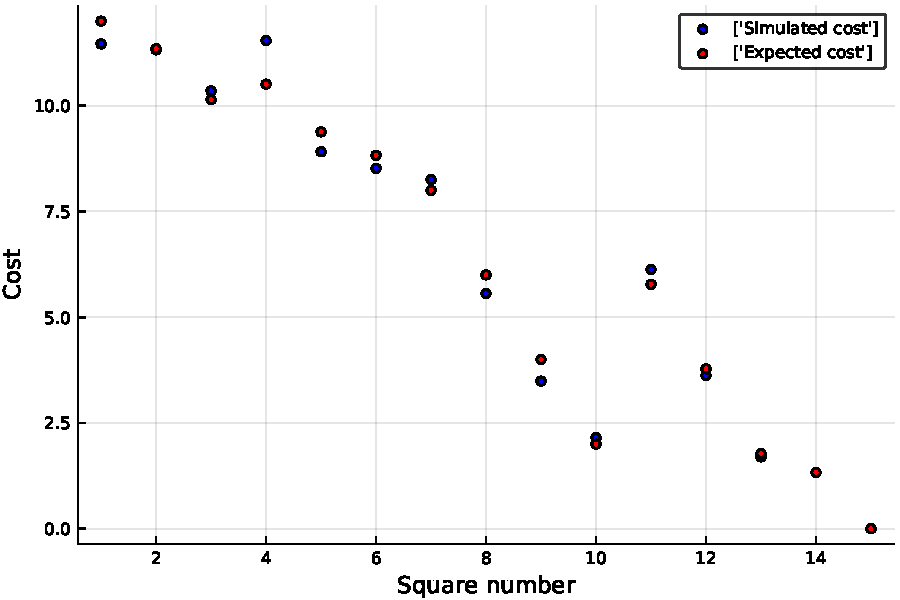
\includegraphics[scale=0.53]{../img/board_right_high/cost_per_square_100_iter_noncirc.pdf}
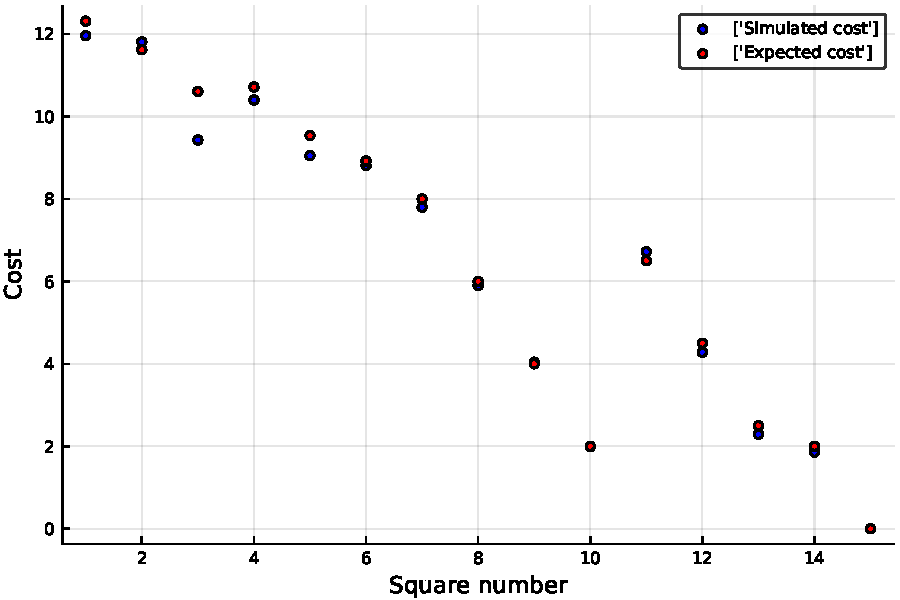
\includegraphics[scale=0.53]{../img/board_right_high/cost_per_square_100_iter_circ.pdf}
\caption{Simulated and expected cost starting from each node for 100 simulations. On the left, results for the non-circular configuration. On the right, the circular one.}
\label{fig:cost_per_square_100_iter_right}
\end{figure}

\begin{figure}[H]
\centering
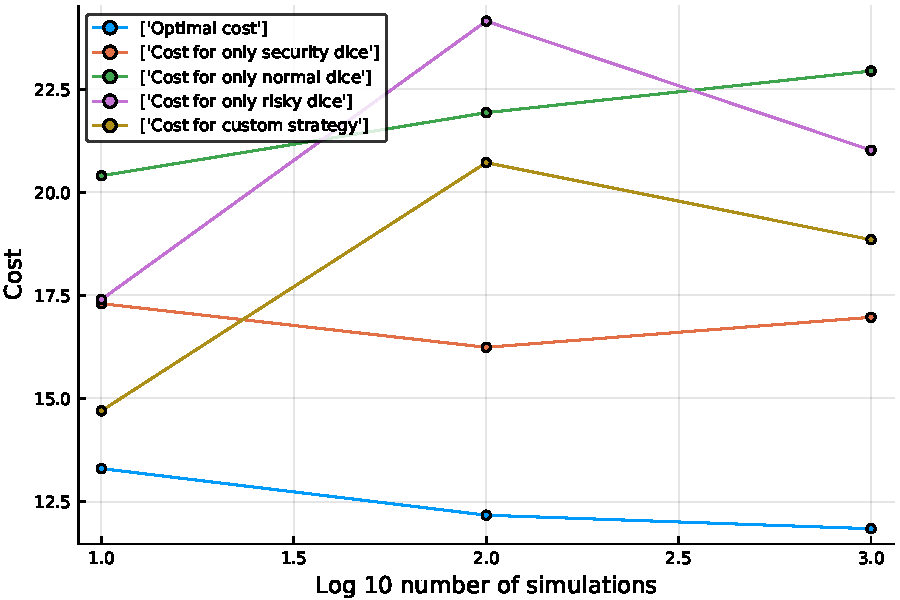
\includegraphics[scale=0.53]{../img/board_right_high/cost_subopt_log_noncirc.pdf}
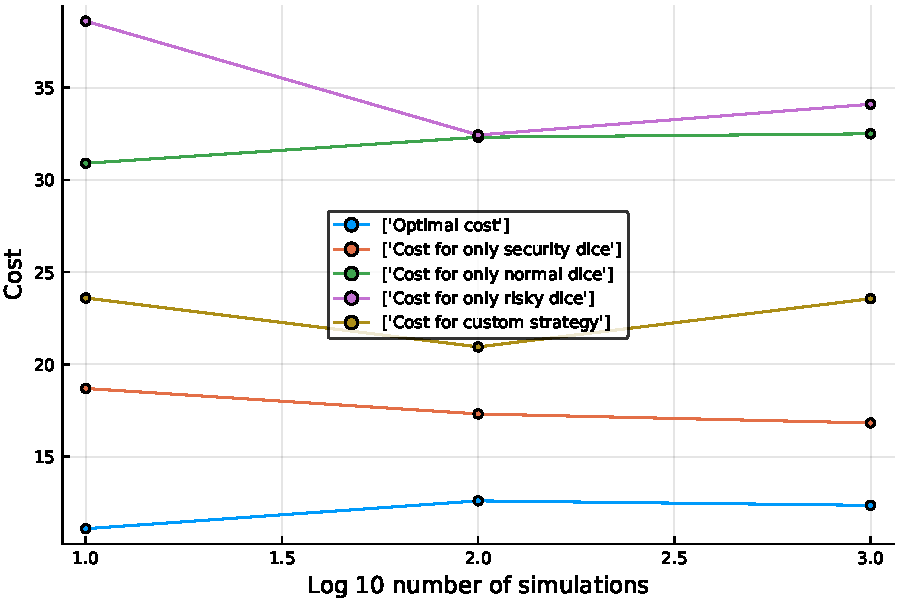
\includegraphics[scale=0.53]{../img/board_right_high/cost_subopt_log_circ.pdf}
\caption{Simulated costs for the different strategies with the number of simulations. On the left, results for the non-circular configuration. On the right, the circular one.}
\label{fig:cost_subopt_log_right}
\end{figure}


\subsection{Left high density trap-distributed board}

The board used in this case is the following (figure~\ref{fig:board_left}).

\begin{figure}[H]
\centering
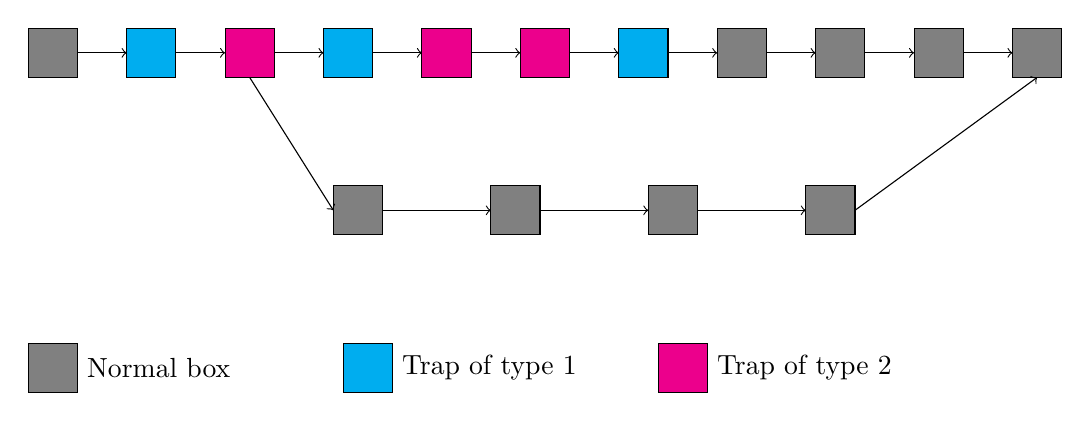
\begin{tikzpicture}[scale=10]
%board = [0,1,2,1,2,2,1,0,0,0,0,0,0,0,0]
\pgfmathsetmacro{\i}{1-1}
\pgfmathsetmacro{\c}{"gray"}
\draw [fill=\c] (2*\i*0.0625,1) rectangle (2*\i*0.0625+0.0625,1-0.0625);
\pgfmathsetmacro{\i}{2-1}
\pgfmathsetmacro{\c}{"cyan"}
\draw [fill=\c] (2*\i*0.0625,1) rectangle (2*\i*0.0625+0.0625,1-0.0625);
\pgfmathsetmacro{\i}{3-1}
\pgfmathsetmacro{\c}{"magenta"}
\draw [fill=\c] (2*\i*0.0625,1) rectangle (2*\i*0.0625+0.0625,1-0.0625);
\pgfmathsetmacro{\i}{4-1}
\pgfmathsetmacro{\c}{"cyan"}
\draw [fill=\c] (2*\i*0.0625,1) rectangle (2*\i*0.0625+0.0625,1-0.0625);
\pgfmathsetmacro{\i}{5-1}
\pgfmathsetmacro{\c}{"magenta"}
\draw [fill=\c] (2*\i*0.0625,1) rectangle (2*\i*0.0625+0.0625,1-0.0625);
\pgfmathsetmacro{\i}{6-1}
\pgfmathsetmacro{\c}{"magenta"}
\draw [fill=\c] (2*\i*0.0625,1) rectangle (2*\i*0.0625+0.0625,1-0.0625);
\pgfmathsetmacro{\i}{7-1}
\pgfmathsetmacro{\c}{"cyan"}
\draw [fill=\c] (2*\i*0.0625,1) rectangle (2*\i*0.0625+0.0625,1-0.0625);
\pgfmathsetmacro{\i}{8-1}
\pgfmathsetmacro{\c}{"gray"}
\draw [fill=\c] (2*\i*0.0625,1) rectangle (2*\i*0.0625+0.0625,1-0.0625);
\pgfmathsetmacro{\i}{9-1}
\pgfmathsetmacro{\c}{"gray"}
\draw [fill=\c] (2*\i*0.0625,1) rectangle (2*\i*0.0625+0.0625,1-0.0625);
\pgfmathsetmacro{\i}{10-1}
\pgfmathsetmacro{\c}{"gray"}
\draw [fill=\c] (2*\i*0.0625,1) rectangle (2*\i*0.0625+0.0625,1-0.0625);
\pgfmathsetmacro{\i}{11-11}
\pgfmathsetmacro{\c}{"gray"}
\draw [fill=\c] (0.45+\i*0.2,0.8) rectangle (0.45+\i*0.2-0.0625,0.8-0.0625);
\pgfmathsetmacro{\i}{12-11}
\pgfmathsetmacro{\c}{"gray"}
\draw [fill=\c] (0.45+\i*0.2,0.8) rectangle (0.45+\i*0.2-0.0625,0.8-0.0625);
\pgfmathsetmacro{\i}{13-11}
\pgfmathsetmacro{\c}{"gray"}
\draw [fill=\c] (0.45+\i*0.2,0.8) rectangle (0.45+\i*0.2-0.0625,0.8-0.0625);
\pgfmathsetmacro{\i}{14-11}
\pgfmathsetmacro{\c}{"gray"}
\draw [fill=\c] (0.45+\i*0.2,0.8) rectangle (0.45+\i*0.2-0.0625,0.8-0.0625);
\pgfmathsetmacro{\i}{15-5}
\pgfmathsetmacro{\c}{"gray"}
\draw [fill=\c] (2*\i*0.0625,1) rectangle (2*\i*0.0625+0.0625,1-0.0625);

\foreach \i in {0,1,...,9}
  \draw [->] (0.0625+2*\i*0.0625,1-0.03125) -- (2*0.0625+2*\i*0.0625,1-0.03125);
\foreach \i in {0,1,2}
  \draw [->] (0.45+\i*0.2,0.8-0.03125) -- (0.45+0.1375+\i*0.2,0.8-0.03125);
\draw [->] (5*0.0625-0.03125,1-0.0625) -- (0.45-0.0625, 0.8-0.03125);
\draw [->] (0.45+0.1375+2*0.2+0.0625,0.8-0.03125) -- (2*10*0.0625+0.0625/2,1-0.0625);

\draw [fill=gray] (0,0.6) rectangle (0.0625, 0.6-0.0625);
\node [right] at (0.0625, 0.6-0.03125) {Normal box};
\draw [fill=cyan] (0.4,0.6) rectangle (0.4 + 0.0625, 0.6-0.0625);
\node [right] at (0.4 + 0.0625, 0.6-0.03125) {Trap of type 1};
\draw [fill=magenta] (0.8,0.6) rectangle (0.8 + 0.0625, 0.6-0.0625);
\node [right] at (0.8 + 0.0625, 0.6-0.03125) {Trap of type 2};
\end{tikzpicture}
\caption{Representation of our high left density trap-distributed board.}
\label{fig:board_left}
\end{figure}

The results graphs are as follows 
(figures~\ref{fig:cost_iterations_log_left}, \ref{fig:cost_per_square_100_iter_left}
and~\ref{fig:cost_subopt_log_left}).

\begin{figure}[H]
\centering
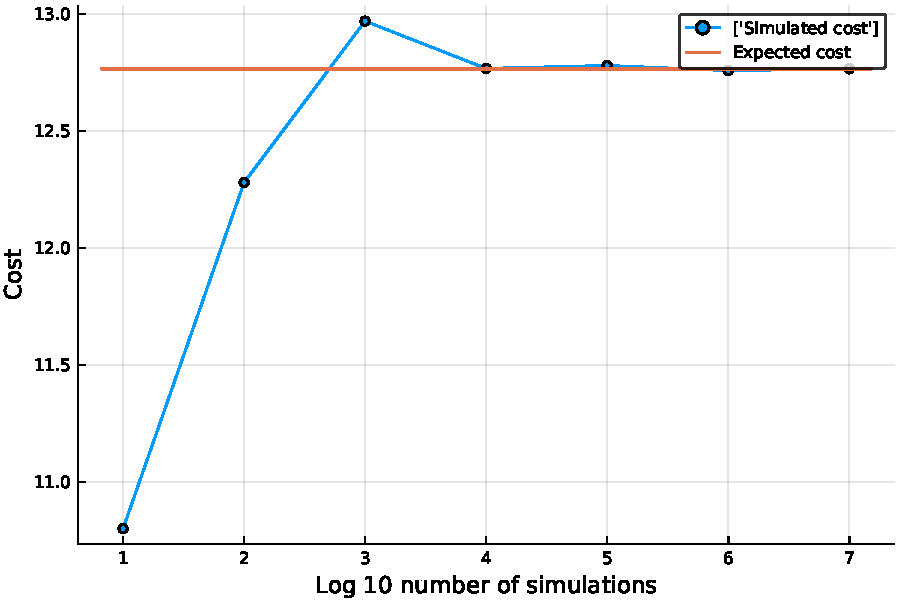
\includegraphics[scale=0.53]{../img/board_left_high/cost_iterations_log_noncirc.pdf}
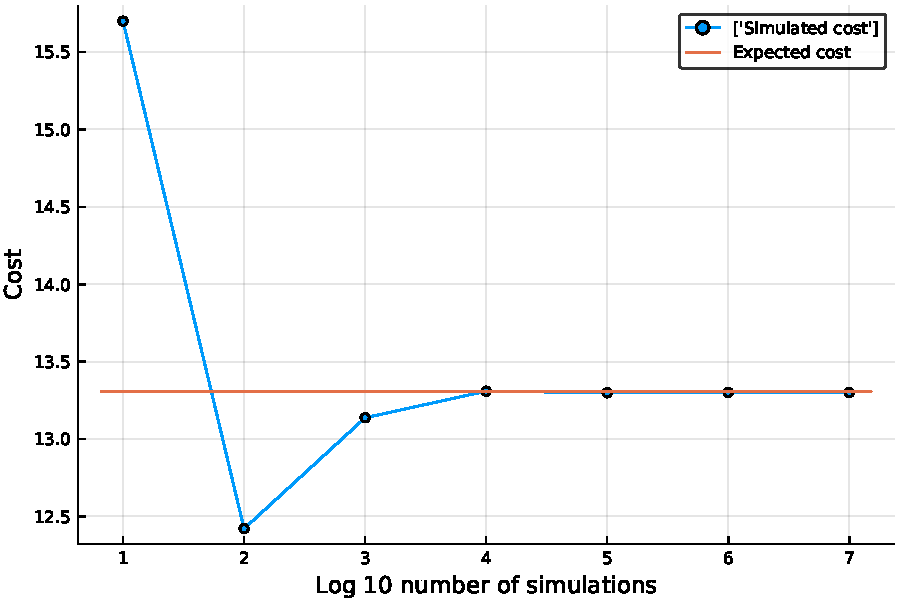
\includegraphics[scale=0.53]{../img/board_left_high/cost_iterations_log_circ.pdf}
\caption{Evolution of the simulated cost with the number of simulations. The horizontal line represent the expected cost computed with the value-iteration algorithm. On the left, results for the non-circular configuration. On the right, the circular one.}
\label{fig:cost_iterations_log_left}
\end{figure}

\begin{figure}[H]
\centering
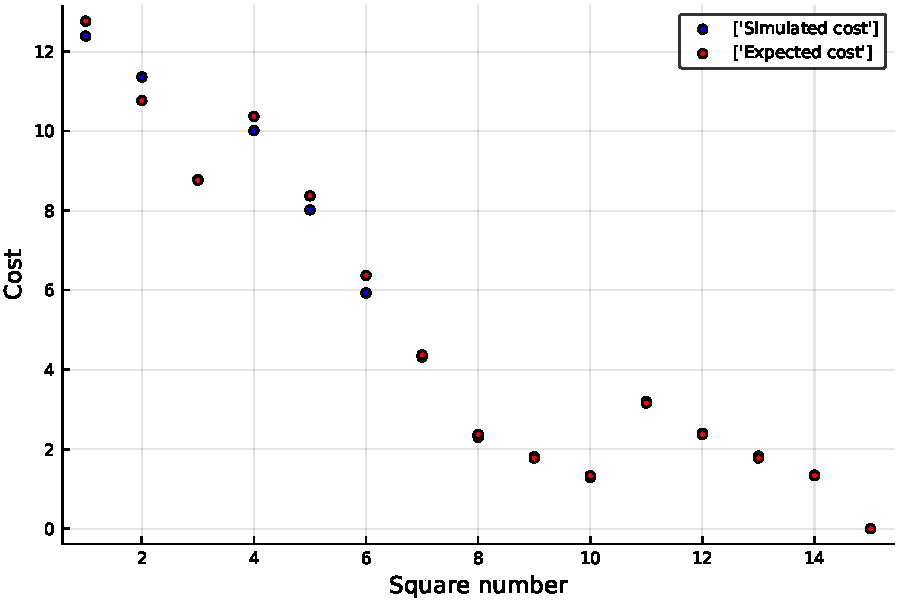
\includegraphics[scale=0.53]{../img/board_left_high/cost_per_square_100_iter_noncirc.pdf}
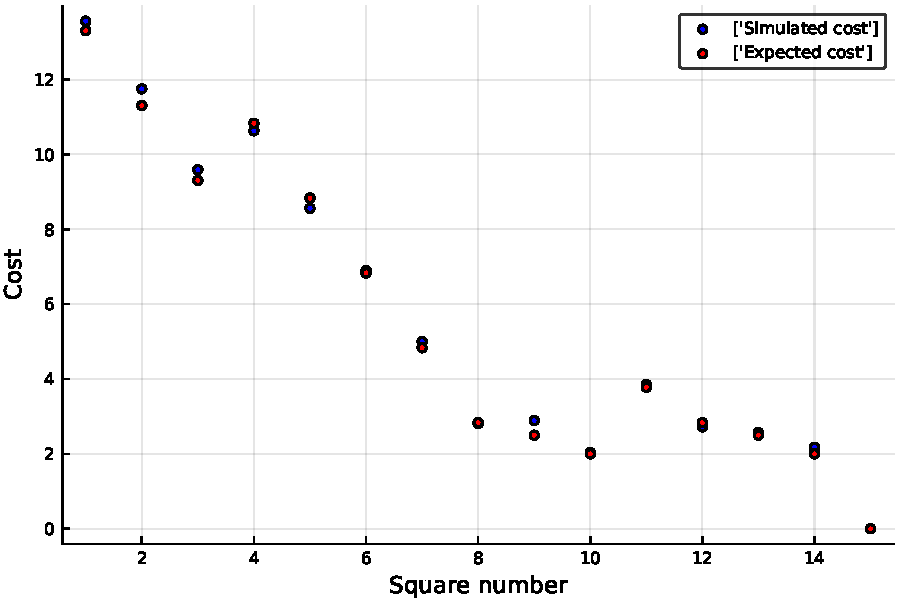
\includegraphics[scale=0.53]{../img/board_left_high/cost_per_square_100_iter_circ.pdf}
\caption{Simulated and expected cost starting from each node for 100 simulations. On the left, results for the non-circular configuration. On the right, the circular one.}
\label{fig:cost_per_square_100_iter_left}
\end{figure}

\begin{figure}[H]
\centering
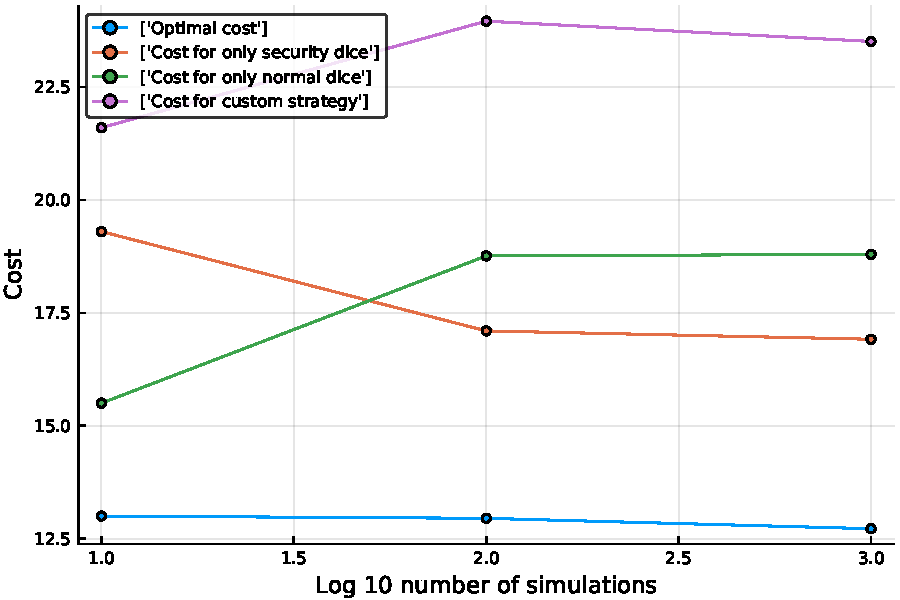
\includegraphics[scale=0.53]{../img/board_left_high/cost_subopt_log_noncirc.pdf}
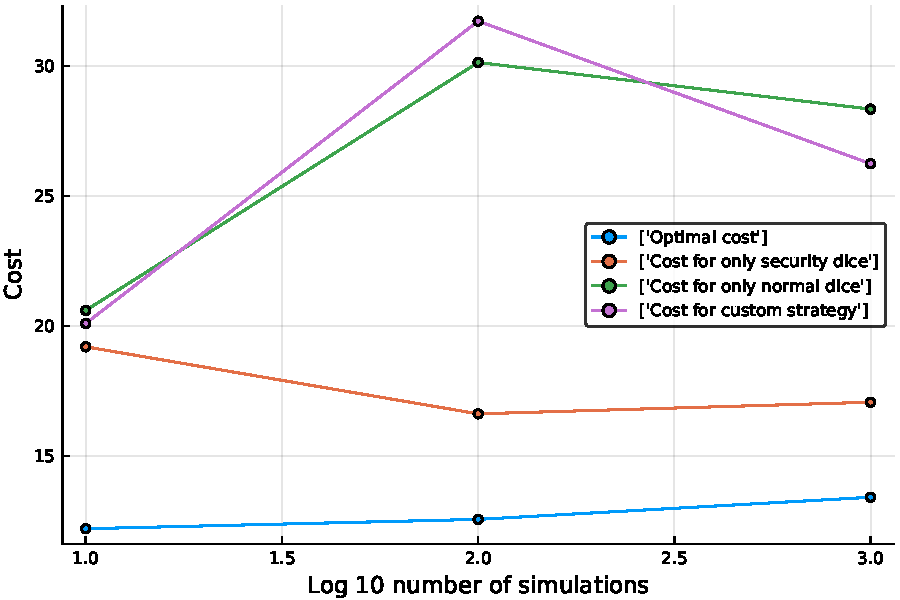
\includegraphics[scale=0.53]{../img/board_left_high/cost_subopt_log_circ.pdf}
\caption{Simulated costs for the different strategies with the number of simulations. On the left, results for the non-circular configuration. On the right, the circular one.}
\label{fig:cost_subopt_log_left}
\end{figure}

\subsection{Magic trap-distributed board}

The board used in this case is the following (figure~\ref{fig:board_magic}).

\vspace{1cm}

\begin{figure}[H]
\centering
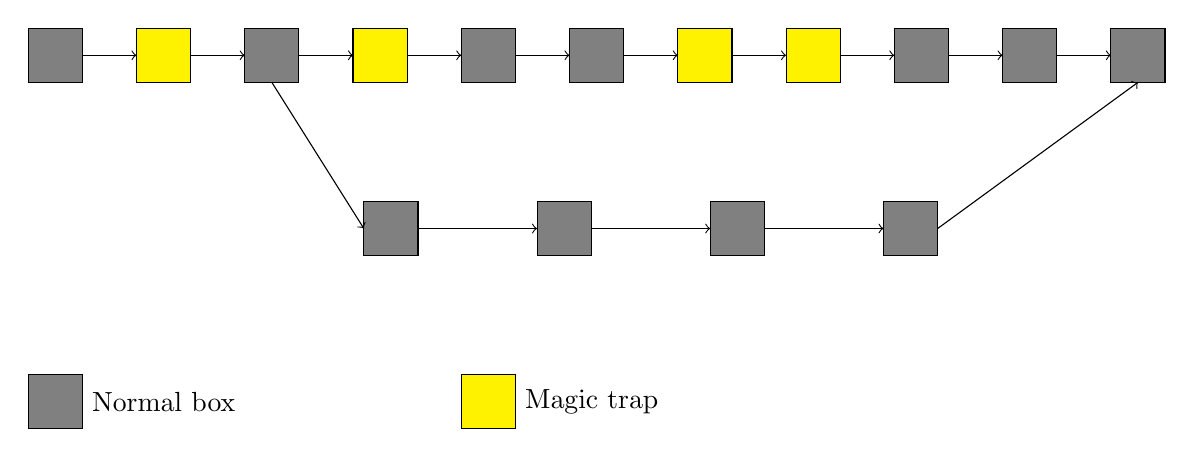
\begin{tikzpicture}[scale=11]
%board = [0,3,0,3,0,0,0,0,3,3,0,0,0,0,0]
\pgfmathsetmacro{\i}{1-1}
\pgfmathsetmacro{\c}{"gray"}
\draw [fill=\c] (2*\i*0.0625,1) rectangle (2*\i*0.0625+0.0625,1-0.0625);
\pgfmathsetmacro{\i}{2-1}
\pgfmathsetmacro{\c}{"yellow"}
\draw [fill=\c] (2*\i*0.0625,1) rectangle (2*\i*0.0625+0.0625,1-0.0625);
\pgfmathsetmacro{\i}{3-1}
\pgfmathsetmacro{\c}{"gray"}
\draw [fill=\c] (2*\i*0.0625,1) rectangle (2*\i*0.0625+0.0625,1-0.0625);
\pgfmathsetmacro{\i}{4-1}
\pgfmathsetmacro{\c}{"yellow"}
\draw [fill=\c] (2*\i*0.0625,1) rectangle (2*\i*0.0625+0.0625,1-0.0625);
\pgfmathsetmacro{\i}{5-1}
\pgfmathsetmacro{\c}{"gray"}
\draw [fill=\c] (2*\i*0.0625,1) rectangle (2*\i*0.0625+0.0625,1-0.0625);
\pgfmathsetmacro{\i}{6-1}
\pgfmathsetmacro{\c}{"gray"}
\draw [fill=\c] (2*\i*0.0625,1) rectangle (2*\i*0.0625+0.0625,1-0.0625);
\pgfmathsetmacro{\i}{7-1}
\pgfmathsetmacro{\c}{"yellow"}
\draw [fill=\c] (2*\i*0.0625,1) rectangle (2*\i*0.0625+0.0625,1-0.0625);
\pgfmathsetmacro{\i}{8-1}
\pgfmathsetmacro{\c}{"yellow"}
\draw [fill=\c] (2*\i*0.0625,1) rectangle (2*\i*0.0625+0.0625,1-0.0625);
\pgfmathsetmacro{\i}{9-1}
\pgfmathsetmacro{\c}{"gray"}
\draw [fill=\c] (2*\i*0.0625,1) rectangle (2*\i*0.0625+0.0625,1-0.0625);
\pgfmathsetmacro{\i}{10-1}
\pgfmathsetmacro{\c}{"gray"}
\draw [fill=\c] (2*\i*0.0625,1) rectangle (2*\i*0.0625+0.0625,1-0.0625);
\pgfmathsetmacro{\i}{11-11}
\pgfmathsetmacro{\c}{"gray"}
\draw [fill=\c] (0.45+\i*0.2,0.8) rectangle (0.45+\i*0.2-0.0625,0.8-0.0625);
\pgfmathsetmacro{\i}{12-11}
\pgfmathsetmacro{\c}{"gray"}
\draw [fill=\c] (0.45+\i*0.2,0.8) rectangle (0.45+\i*0.2-0.0625,0.8-0.0625);
\pgfmathsetmacro{\i}{13-11}
\pgfmathsetmacro{\c}{"gray"}
\draw [fill=\c] (0.45+\i*0.2,0.8) rectangle (0.45+\i*0.2-0.0625,0.8-0.0625);
\pgfmathsetmacro{\i}{14-11}
\pgfmathsetmacro{\c}{"gray"}
\draw [fill=\c] (0.45+\i*0.2,0.8) rectangle (0.45+\i*0.2-0.0625,0.8-0.0625);
\pgfmathsetmacro{\i}{15-5}
\pgfmathsetmacro{\c}{"gray"}
\draw [fill=\c] (2*\i*0.0625,1) rectangle (2*\i*0.0625+0.0625,1-0.0625);

\foreach \i in {0,1,...,9}
  \draw [->] (0.0625+2*\i*0.0625,1-0.03125) -- (2*0.0625+2*\i*0.0625,1-0.03125);
\foreach \i in {0,1,2}
  \draw [->] (0.45+\i*0.2,0.8-0.03125) -- (0.45+0.1375+\i*0.2,0.8-0.03125);
\draw [->] (5*0.0625-0.03125,1-0.0625) -- (0.45-0.0625, 0.8-0.03125);
\draw [->] (0.45+0.1375+2*0.2+0.0625,0.8-0.03125) -- (2*10*0.0625+0.0625/2,1-0.0625);

\draw [fill=gray] (0,0.6) rectangle (0.0625, 0.6-0.0625);
\node [right] at (0.0625, 0.6-0.03125) {Normal box};
\draw [fill=yellow] (0.5,0.6) rectangle (0.5 + 0.0625, 0.6-0.0625);
\node [right] at (0.5 + 0.0625, 0.6-0.03125) {Magic trap};
\end{tikzpicture}
\caption{Representation of our magic board.}
\label{fig:board_magic}
\end{figure}

\vspace{3cm}

The results graphs are as follows 
(figures~\ref{fig:cost_iterations_log_magic}, \ref{fig:cost_per_square_100_iter_magic}
and~\ref{fig:cost_subopt_log_magic}).

\vspace{1cm}

\begin{figure}[H]
\centering
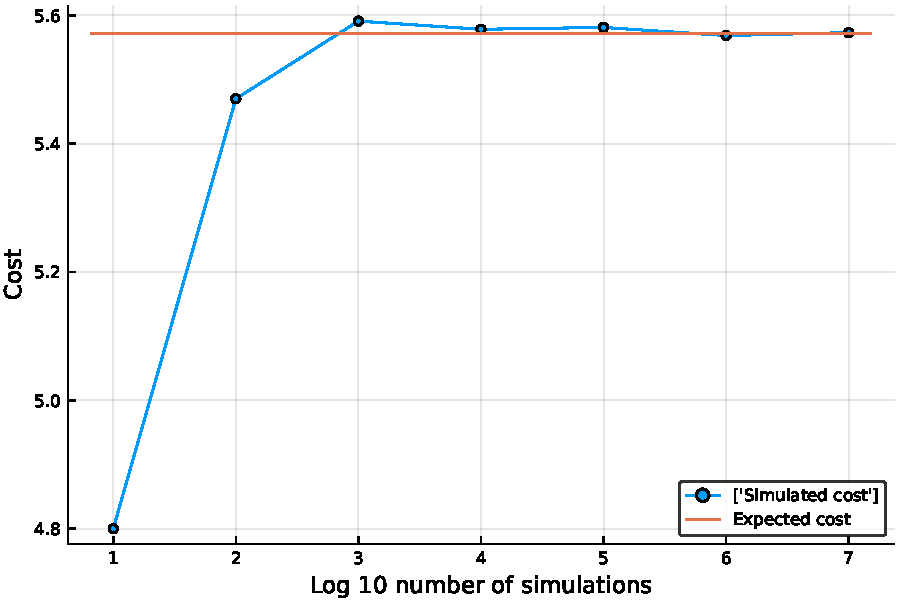
\includegraphics[scale=0.53]{../img/board_magic/cost_iterations_log_noncirc.pdf}
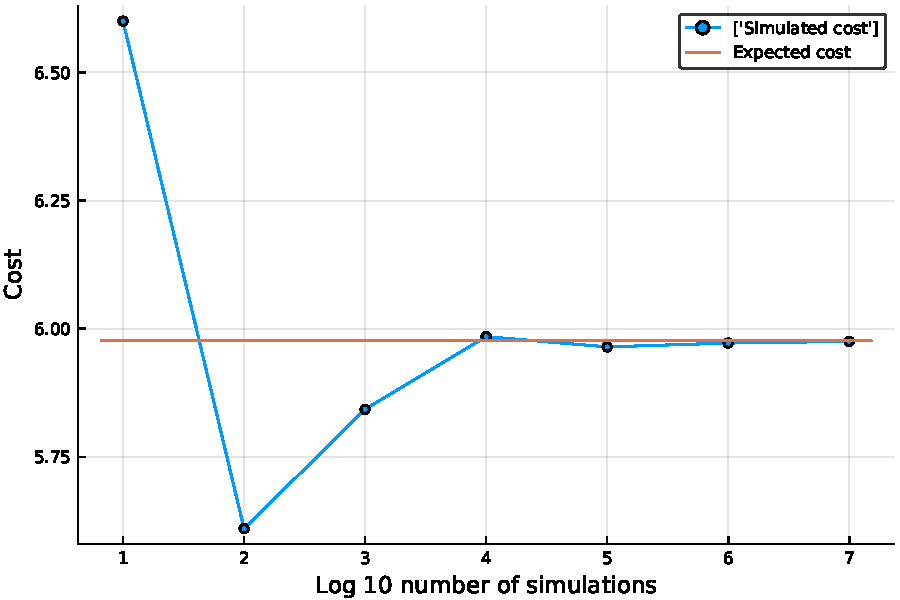
\includegraphics[scale=0.53]{../img/board_magic/cost_iterations_log_circ.pdf}
\caption{Evolution of the simulated cost with the number of simulations. The horizontal line represent the expected cost computed with the value-iteration algorithm. On the left, results for the non-circular configuration. On the right, the circular one.}
\label{fig:cost_iterations_log_magic}
\end{figure}

\begin{figure}[H]
\centering
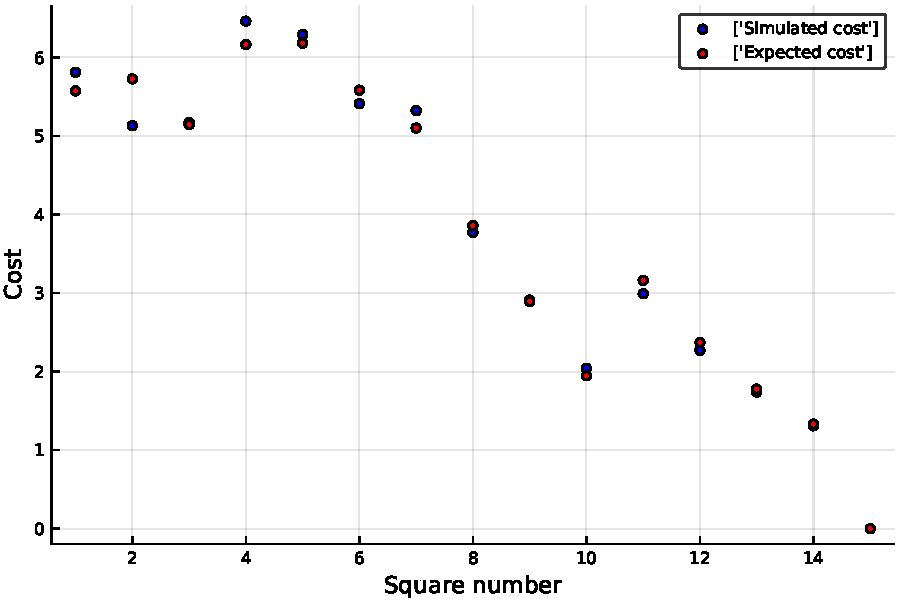
\includegraphics[scale=0.53]{../img/board_magic/cost_per_square_100_iter_noncirc.pdf}
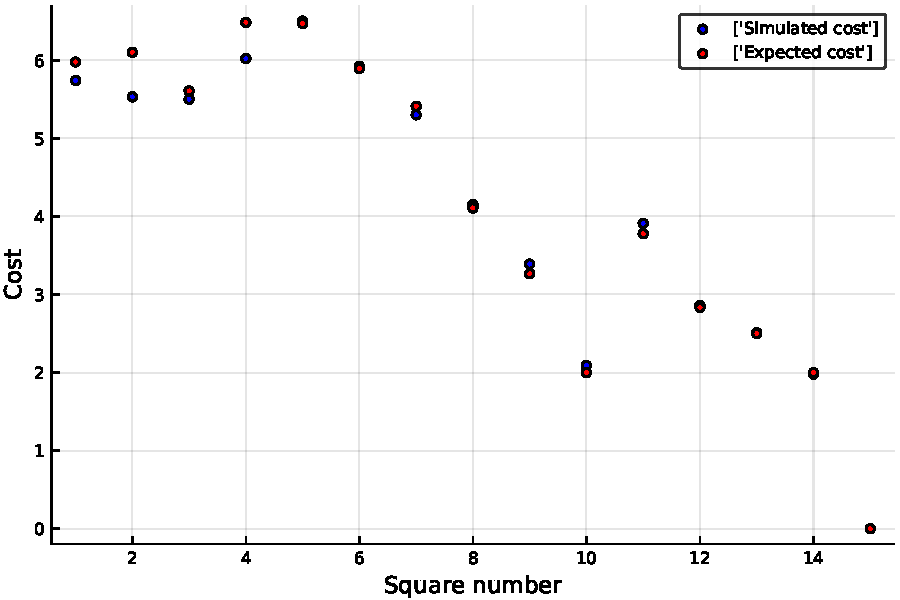
\includegraphics[scale=0.53]{../img/board_magic/cost_per_square_100_iter_circ.pdf}
\caption{Simulated and expected cost starting from each node for 100 simulations. On the left, results for the non-circular configuration. On the right, the circular one.}
\label{fig:cost_per_square_100_iter_magic}
\end{figure}

\begin{figure}[H]
\centering
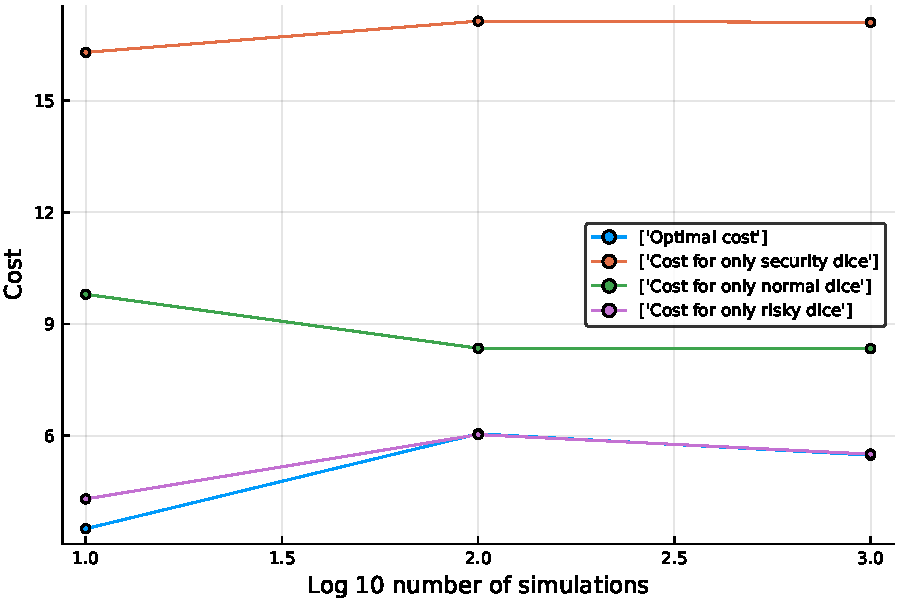
\includegraphics[scale=0.53]{../img/board_magic/cost_subopt_log_noncirc.pdf}
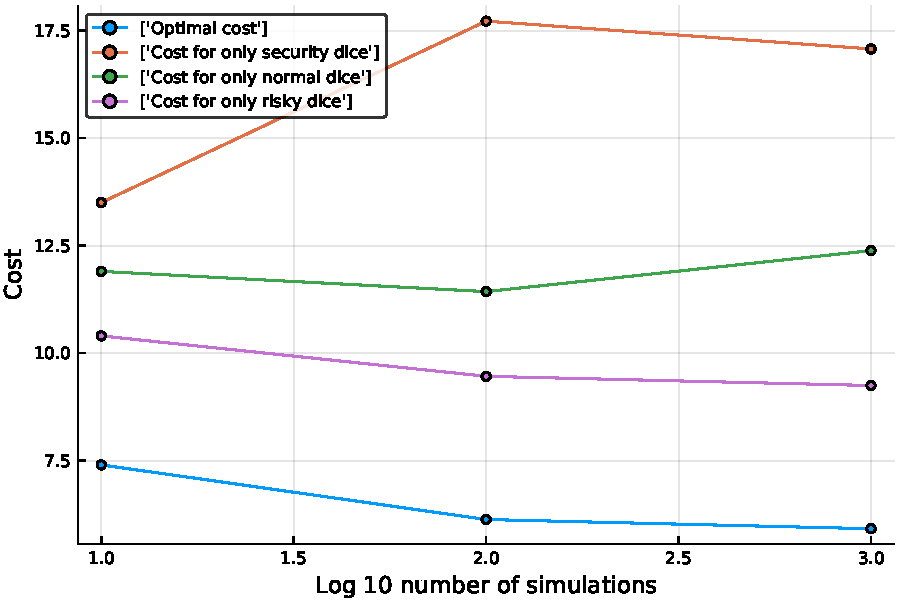
\includegraphics[scale=0.53]{../img/board_magic/cost_subopt_log_circ.pdf}
\caption{Simulated costs for the different strategies with the number of simulations. On the left, results for the non-circular configuration. On the right, the circular one.}
\label{fig:cost_subopt_log_magic}
\end{figure}
% section additional_error_plots (end)